\documentclass[12pt]{article}

\usepackage[letterpaper,total={7in,10in}]{geometry}
\usepackage{tikz}
\usepackage{graphicx}
\usepackage{ragged2e}
\usepackage{listings}
\usepackage{color}
\usepackage{multicol}
\usepackage{hyperref}

\renewcommand{\ttdefault}{txtt}
\renewcommand{\familydefault}{\ttdefault}

\lstset{backgroundcolor = \color[rgb]{0.88, 0.88, 0.96}}
\lstset{numbers = left}
\lstset{breaklines = true}
\begin{document}
	\Centering \huge \textbf{\underline{Programming Dictionary}}

	\Large By Charles Cook

	\large Begun on Dec. 6th, 2018

	\FlushLeft \normalsize \tableofcontents

	\section{Compiler Theoretical Foundations} \large
	\Centering 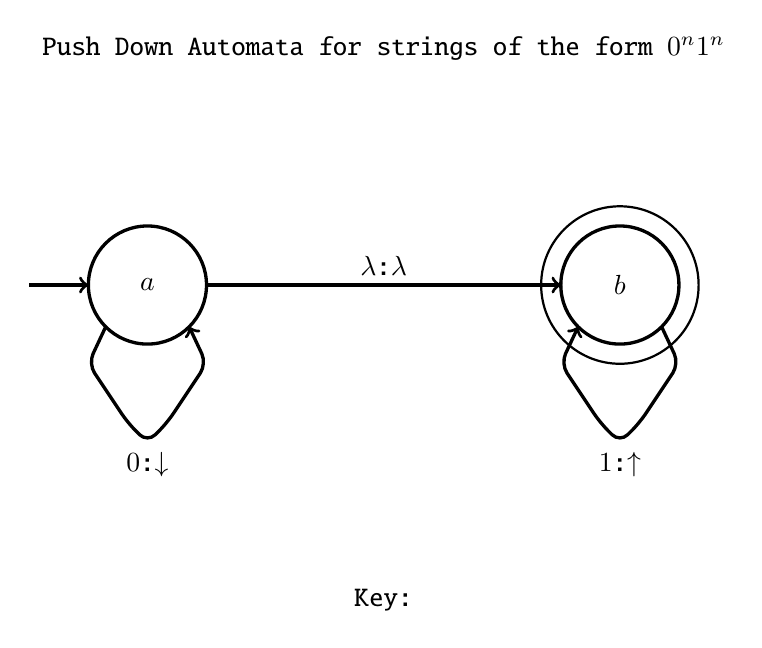
\begin{tikzpicture}
		\node at (0, 3) {Push Down Automata for strings of the form $0^n1^n$};
		\draw [very thick, ->] (-4.5, 0) -- (-3.75, 0);
		\draw [very thick] (-3, 0) circle (0.75);
		\node at (-3, 0) {$a$};
		\draw [very thick, rounded corners, ->] (-3.53, -0.53) -- (-3.75, -1) -- (-3.25, -1.75) -- (-3, -2) -- (-2.75, -1.75) -- (-2.25, -1) -- (-2.47, -0.53);
		\node [below] at (-3, -2) {$0$:$\downarrow$};
		\draw [very thick, ->] (-2.25, 0) -- (2.25, 0);
		\node [above] at (0, 0) {$\lambda$:$\lambda$};
		\draw [very thick] (3, 0) circle (0.75);
		\draw [thick] (3, 0) circle (1);
		\node at (3, 0) {$b$};\draw [very thick, rounded corners, ->] (3.53, -0.53) -- (3.75, -1) -- (3.25, -1.75) -- (3, -2) -- (2.75, -1.75) -- (2.25, -1) -- (2.47, -0.53);
		\node [below] at (3, -2) {$1$:$\uparrow$};
		\node at (0, -4) {Key:};
	\end{tikzpicture}

	\begin{tabular}{|l||r|}
		\hline Symbol & Meaning \\ \hline
		$a$, $b$ & State Node \\ \hline
		$0$, $1$ & Symbol to Print \\ \hline
		$\downarrow$ & Push (onto the stack) \\ \hline
		$\uparrow$ & Pull (off of the stack) \\ \hline
		$\lambda$ & Null operation \\ & (no print, push, or pull) \\ \hline
	\end{tabular} \linebreak

	Derivation Examples: $01$, $00001111$, $0000000011111111$.

	\pagebreak

	\FlushLeft \normalsize
	\section{Programming Tools \& Languages: First Ten Questions}
	\subsection{Swap Function}
	\subsubsection{Pseudocode for \textit{swap}}
	\begin{lstlisting}[language = C, tabsize = 8]
void swap(a, b) {
	temp = a;
	a = b;
	b = temp;
}

void swapNoTemp(a, b) {
	a += b; // a = a + b
	b -= a; // b = b - (a + b) = -a
	b *= -1; // b = a
	a -= b; // a = a + b - a = b
}
	\end{lstlisting}

	\subsubsection{\textit{swaptest.c}}
	\begin{lstlisting}[language = C, showstringspaces = false, tabsize = 8]
#include <stdio.h>
void swap(int *a, int *b) {
	*a += *b;
	*b -= *a;
	*b *= -1;
	*a -= *b;
}

int main() {
	int x, y, z;
	x = 10;
	y = 13;
	z = 2;

	swap(&x, &y);
	swap(&x, &z);
	swap(&y, &z);
	printf("x: &d\ny: &d\nz: &d\n", x, y, z);

	return 0;
}
	\end{lstlisting}
	\pagebreak
	\subsubsection{\textit{swaptest.cpp}}
	\begin{lstlisting}[language = C++, showstringspaces = false, tabsize = 8]
#include <iostream>
using namespace std;

void swap(int *a, int *b) {
	*a += *b;
	*b -= *a;
	*b *= -1;
	*a -= *b;
}

int main() {
	int x, y;
	x = 13;
	y = 29;

	cout << x << ", " << y << "\n";
	swap(x, y);
	cout << x << ", " << y << "\n";

	return 0;
}
	\end{lstlisting}

	\subsection{Reverse an array with no extra space (pseudocode)}
	\begin{lstlisting}[language = C, showstringspaces = false, tabsize = 8]
void reverseArray(array, int length) {
	for (int i = 0; i < length / 2; i++) {
		swap(array[i], array[length - i - 1]);
	}
}
	\end{lstlisting}

	\subsection{Reverse a doubly linked list (pseudocode)}
	\begin{lstlisting}[language = C, showstringspaces = false, tabsize = 8]
struct Node {
	int data;
	struct Node *next;
	struct Node *prev;
};

void reverseDLL(head, tail) {
	struct Node tempH = head;
	struct Node tempT = tail;

	while (tempH -> next != tempT -> prev && tempH != tempT) {
		swap(tempH -> data, tempT -> data);
	}
}
	\end{lstlisting}
	\subsection{Reverse a doubly linked list recursively (pseudocode)}
	\begin{lstlisting}[language = C, showstringspaces = false, tabsize = 8]
void reverseDLL_Recursive(head, tail) {
	if (head -> next != tail -> prev && head != tail) {
		swap(head -> data, tail -> data);
		reverseDLL_Recursive(head -> next, tail -> prev);
	}
}
	\end{lstlisting}
	\subsection{Pointer to a Pointer}
	A use of a pointer-to-a-pointer in C would be to insert an element into a sorted singly-linked list. Take the following list:

	\begin{lstlisting}
head:
 [2] -> [4] -> [7] -> [10] -> [13]
	\end{lstlisting}

	Say we want to insert the node \textbf{[9]} into the list; If we make a pointer-to-pointer, call it \textbf{pp}, and make it point to the \textbf{next} attribute of each node, we can insert \textbf{[9]} as follows: \linebreak

	First, we set the value of \textbf{pp} to be the \textbf{head} of the list: \linebreak

	\textbf{*pp = head;} \linebreak

	where head is the pointer to the first struct in the list. We can visualize this below:

	\begin{lstlisting}
 pp
  |
  V
head:
 [2] -> [4] -> [7] -> [10] -> [13]
	\end{lstlisting}

	\textbf{*pp} is \textbf{[2]}, and \textbf{[2] -> data} is 2, which is less than 9. Until we find a candidate \textbf{*pp -> data} that is greater than 9, we keep going by setting \textbf{pp} to the address of the next node with \textbf{*pp = \&(*pp -> next)}.

	\begin{lstlisting}
 pp -+
     |
head:V
 [2] -> [4] -> [7] -> [10] -> [13]
	\end{lstlisting}

	\textbf{*pp} is \textbf{[2] -> next} which is \textbf{[4]}, \textbf{[4] -> data} is 4 which is less than 9, keep going; \textbf{*pp = \&(*pp -> next)}

	\begin{lstlisting}
 pp --------+
            |
head:       V
 [2] -> [4] -> [7] -> [10] -> [13]
	\end{lstlisting}

	\textbf{*pp} is \textbf{[4] -> next} which is \textbf{[7]}, \textbf{[7] -> data} is 7 which is less than 9, keep going; \textbf{*pp = \&(*pp -> next)}

	\begin{lstlisting}
 pp ---------------+
                   |
head:              V
 [2] -> [4] -> [7] -> [10] -> [13]
	\end{lstlisting}

	Paydirt! \textbf{*pp -> data} is 10, which is greater than 9. Now we do the following: \linebreak

	\textbf{[9] -> next = *pp;}

	\begin{lstlisting}
 pp ---------------+
                   |
head:              V
 [2] -> [4] -> [7] -> [10] -> [13]
                      ^
                      |
                 [9] -+
\end{lstlisting}

	\textbf{*pp = [9];}

	\begin{lstlisting}
 pp ---------------+
                   |
head:              V
 [2] -> [4] -> [7] -+ [10] -> [13]
                   /  ^
                  V   |
                 [9] -+
\end{lstlisting}

	The list is still ordered, and \textbf{pp} is needed no longer.

	\subsection{Sorting Algorithm with $O(n)$ Complexity}
	An optimised Bubble Sort that stops after doing a pass thru an array wherein no swaps occur will run in $O(n)$ time on an already-sorted list. In a sorted list, comparing every element with its next element all the way to the end will not prompt Bubble Sort to perform any swaps at all. When a single pass of the array is completed and no swaps have occured, a proper Bubble Sort will stop, as no swaps is a sign of a sorted list.

	\subsection{Selection Sort Complexity}
	Consider the worst case of Selection Sort: a completely-reversed array, say $(6, 5, 4, 3, 2, 1)$. On the first pass, $1$ is selected, and has to be moved $5$ indices, $n - 1$. On the second pass, $2$ is selected, and has to be moved $4$ indices, $n - 2$. This eventually boils down to $n - 1 + n - 2 + n - 3 + n - 4 + n - 5$ operations; given $n = 6$, this becomes $6 - 1 + 6 - 2 + 6 - 3 + 6 - 4 + 6 - 5 = 5 + 4 + 3 + 2 + 1 = 5 * 6 / 2$ (per Gauss' Formula). If we reintroduce $n$, we get $\frac{(n - 1) * n}{2} = \frac{n^2 - n}{2}$. Overall, Selection Sort's worst case (and average case) boils down to $O(n^2)$.

	\subsection{Insertion Sort Complexity}
	Consider again $(6, 5, 4, 3, 2, 1)$. On the first pass of Insertion Sort, the $5$ is swapped $1$ time, $n - 5$. On the second pass, the $4$ is swapped $2$ times, $n - 4$. Note the pattern. Overall, there are $n - 5 + n - 4 + n - 3 + n - 2 + n - 1$. Recall from the previous problem on Selection Sort that this boils down to $\frac{(n - 1)n}{2} = \frac{n^2 - n}{2}$. Insertion Sort is also worst-case and average-case $O(n^2)$ complexity.

	\subsection{\textit{ordered} Predicate in Prolog}
	\subsubsection{\textit{sorted.pl}}
	\begin{lstlisting}[language = Prolog]
ordered([X]).
ordered([X, Y|Z]) :- X < Y, ordered([Y|Z]).
	\end{lstlisting}

	\subsubsection{Output on $[1, 2, 4, 8, 16]$ with trace-on in GProlog}
	\begin{lstlisting}
| ?- ordered([1,2,4,8,16]).
      1    1  Call: ordered([1,2,4,8,16]) ?
      2    2  Call: 1<2 ?
      2    2  Exit: 1<2 ?
      3    2  Call: ordered([2,4,8,16]) ?
      4    3  Call: 2<4 ?
      4    3  Exit: 2<4 ?
      5    3  Call: ordered([4,8,16]) ?
      6    4  Call: 4<8 ?
      6    4  Exit: 4<8 ?
      7    4  Call: ordered([8,16]) ?
      8    5  Call: 8<16 ?
      8    5  Exit: 8<16 ?
      9    5  Call: ordered([16]) ?
      9    5  Exit: ordered([16]) ?
      7    4  Exit: ordered([8,16]) ?
      5    3  Exit: ordered([4,8,16]) ?
      3    2  Exit: ordered([2,4,8,16]) ?
      1    1  Exit: ordered([1,2,4,8,16]) ?

true ?

yes
{trace}
| ?-
	\end{lstlisting}
	\pagebreak

	\subsection{Labelled Path (with cost) in Prolog}
	\subsubsection{ASCII-art chart of my path}
	\begin{lstlisting}
                           +-[11]-> (d) -[7]-> (f)
(a) -[1]-> (b) -[3]-> (c) -+
                           +-[5]-> (e) -+-[13]-> (g)
                                        |
                                        +-[19]-> (h)
	\end{lstlisting}

	\subsubsection{\textit{charliesPath.pl}}
	\begin{lstlisting}[language = Prolog, tabsize = 8]
link(a, b, 1).
link(b, c, 3).
link(c, d, 11).
link(c, e, 5).
link(d, f, 7).
link(e, g, 13).
link(e, h, 19).

path(Origin, Destination, Distance) :-
	link(Origin, Destination, Distance)
.
path(Origin, Destination, TotalDistance) :-
	link(Origin, Intermediate, DistanceA),
	path(Intermediate, Destination, DistanceB),
	TotalDistance is DistanceA + DistanceB
.
	\end{lstlisting}

	\subsubsection{Recursion Analysis}
	Whenever path is called with two locations that are indirectly linked, the first thing that will happen is that all directly linked locations to the Origin will be checked; these are the Intermediate locations. These locations will eached be checked to see if they have a direct link to the Destination, otherwise their directly linked locations will act as new Intermediates and themselves go through the same check. \linebreak

	Once an Intermediate is found that directly connects to the Destination, the recursion will cease and the value of true will be returned, along with the total distance. If all recursion becomes exhausted and no satisfactory Intermediate is found, the value of false will be returned.
	\pagebreak

	\section{Programming Tools \& Languages: Last Ten Questions}
	\subsection{Number of nodes in a linked list (pseudocode)}
	\begin{lstlisting}[language = C, tabsize = 8]
int numberOfNodes(head) {
	int n = 1;
	temp = head;

	while (temp -> next != NULL) {
		n += 1;
		temp = temp -> next;
	}

	return n;
}
	\end{lstlisting}

	\subsection{Number of nodes in a linked list (pseudocode, $O(\frac{n}{2})$ complexity)}
	\begin{lstlisting}[language = C, tabsize = 8]
int numberOfNodesQuick(head) {
	int n = 1;
	temp = head;

	while (temp -> next != NULL && temp -> next -> next != NULL) {
		n += 2;
		temp = temp -> next -> next;
	}

	if (temp -> next != NULL) {
		n += 1;
	}

	return n;
}
	\end{lstlisting}

	\subsection{Return middle node of linked list (pseudocode)}
	\begin{lstlisting}[language = C, tabsize = 8]
node middleNode(head, int length) {
	temp = head;

	for (int i = 0; i < length / 2; i++) {
		temp = temp -> next;
	}

	return temp;
}
	\end{lstlisting}

	\subsection{Return middle node of linked list with two pointers}
	Declare two pointers and initialize them with the head value. Let the first pointer be known as the one-jump, and the second as the two-jump. While the two-jump pointer's next is not equal to NULL and it's next-next is not equal to NULL, have the one-jump pointer take on the next value one node ahead, and have the two-jump pointer take on the next value two nodes ahead. When the two-jump has a next that is NULL, the one-jump will be in the middle. \linebreak

	For example, if a linked list has $9$ nodes, the two-jump will go from node $1$ to $3$ to $5$ to $7$ to $9$, then stop. The one-jump will go from node $1$ to $2$ to $3$ to $4$ to $5$, then stop. $5$ is halfway between node $1$ and node $9$.

	\subsection{Circualr singly-linked list check with two pointers}
	Declare two pointers as before when finding the middle node of a linked list: one-jump and two-jump. A circular linked list can be detected if you repeatedly have the one-jump update to its next node, and have the two-jump update to its next-next node. If ever the nodes ever are equal, i.e. they are pointing to the same node, then there is a cycle in the list. If there wasn't, the two-jump would reach a terminal point well ahead of the one-jump.

	\subsection{Reachability}
	It is possible to run a reachability function on a directed graph / linked list map that runs in polynomial time. For this, we need an array, identified as $marked$, and a stack, identified as $reached$. Starting from the root node of travel, push this node onto $reached$. Then, begin a loop which will continue until $reached$ is empty, or until the desired node to reach gets pushed to $reached$. In each pass, if the top element in $reached$ has children, pop it off and append its address a.k.a. indentifier to $marked$. Then, push all of its child nodes onto $reached$, except those already in $marked$. This condition prevents a cyclic map from running the algorithm forever. \linebreak

	As the loop proceeds, eventually all ultimate child nodes will be pushed to the stack. If the top node at the start of a pass has no children, then pop it off and start a new pass of the loop. If only ultimate children are in the stack, and none of them are the desired node, then $reached$ will be emptied, and a $false$ value can be returned. If the node-to-be-reached is ever pushed to $reached$ however, then a $true$ value can be returned. With the $marked$ array, no node will ever be pushed to $reached$ twice, which makes this a P-class algorithm. \pagebreak

	\subsection{Stable vs. Non-Stable Sorting Algorithms}
	A stable sorting algorithm is one that preserves the order of elements of equal value from before sorting to after sorting. Insertion Sort is stable, because when an equal value element is inserted, it will not be able to move beyong another equal value element, because the citeria for an insertion swap requires the lower element to be strictly less than the higher element. Selection Sort, in its simplest implementation, is not stable. If a minimum finding function that uses a linear search is used, the last instance of an equal value element will become the first instance, breaking stability.

	\subsection{Fundamental Data Structures}
	\begin{itemize}
		\item Array
		\item Dictionary (a.k.a. Hash Table, Associative Array)
		\item Linked List (singly or doubly linked)
		\item Binary Search Tree (Lefthand children are smaller, righthand are larger)
		\item Heap Tree (In a maximum heap, all children are smaller)
		\item Stack
	\end{itemize}

	\subsection{P vs. NP}
	The "P" in P vs. NP stands for polynomial. If an algorithm qualifies for a P-class problem, then the Big-$O$ complexity of the algorithm is modelled by a polynomial expression; In short, the algorithm runs in polynomial-class time in reference to the size of the input. Alternatly, if an algorithm is of the NP-class, its time complexity is non-polynomial, which is ususally worse than polynomial complexity. For example, there are only NP-class algorithms for solutions to the Travelling Salesman Problem, which entales travelling to every node in a graph (every city in a region) and returning to your starting location while minimizing distance.

	\subsection{Class vs. Struct}
	A struct is a composite data type with multiple data fields of any type defined in the programming language. A class combines the data-ordering of a struct with associated functions called methods, which manipulate the data ordered by the class. When a class is instantiated, the instance is referred to as an object.
	\pagebreak

	\section{Palindromes in Prolog}
	\subsection{palindrome.pl}
	\begin{lstlisting}[language = Prolog, tabsize = 8]
concat([], L, L).
concat([X|L1], L2, [X|L3]) :- concat(L1, L2, L3).
reverselist([], []).
reverselist([Head|Tail], Reversed) :-
	reverselist(Tail, ReversedTail),
	concat(ReversedTail, [Head], Reversed)
.
palindrome(X) :- reverselist(X, X).
	\end{lstlisting}
	\subsection{Analysis}
	\subsubsection{concat()}
	The three parameters in concat() are the lefthand list, the righthand list, and the concatenated list. Clearly, the concatenated list is where all the lefthand list's elements are added first, then followed by the elements of the righthand list. As seen in the second statement, To concatenate $[X|L_1]$ with $L_2$, $L_1$ and $L_2$ have to concatenate to $L_3$, which results in $[X|L_3]$. Eventually, after enough recursive calls, $L_1$ will be an empty list, in which case the first statement will be invoked, returning $L_2$ back up the stack.

	\subsubsection{reverselist()}
	The two parameters in reverselist() are the original list, $[Head|Tail]$, and the reversed list, $Reversed$. First, a recursive call is issued with $Tail$ and $ReversedTail$ as the parameters. Second, the recursive call is conjucted with a concat() call of $ReversedTail$ with $[Head]$, which results in $Reveresed$. Back to the first call, the $Tail$ will repeatedly be widdled down until it is empty, which will fulfill the statement that an empty list is the reverse of itself. When this happens, the final element will be in $ReversedTail$ in the highest call (stack-wise) will be concatenated to the element before it, and this will cascade down the stack of calls, completing the $Reversed$ list.

	\subsubsection{palindrome()}
	A palindrome is any ordered arrangement that is its own reverse. Thus, if a call of reverselist() is issued with $X$ and $X$ as both parameters, and the end result is true, then $X$ is a palindrome.
	\pagebreak

	\section{My Project: Visualized Sorting Algorithms Demonstration}
	\Centering
	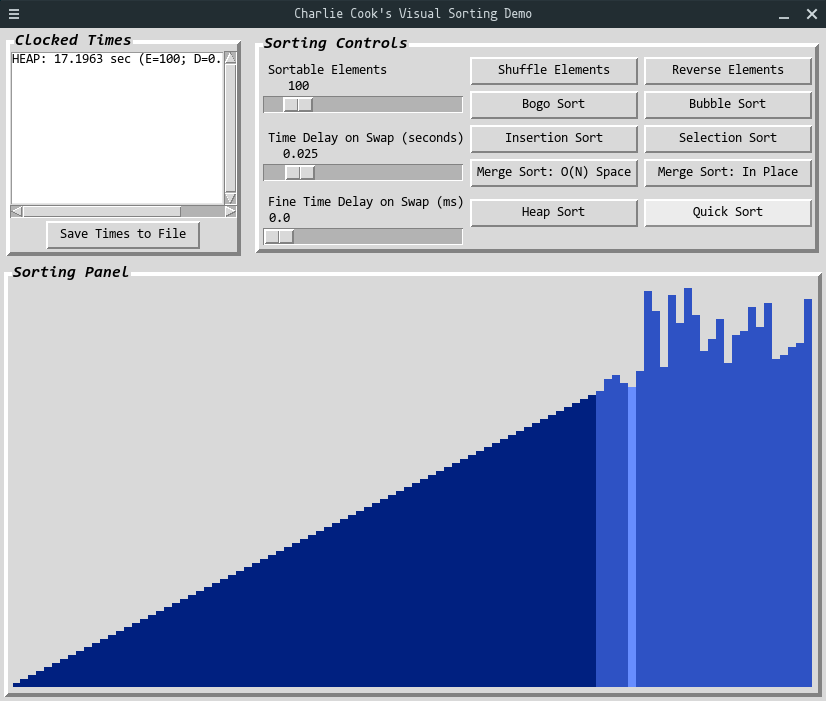
\includegraphics[width = 0.8\linewidth]{sortingdemo.png}
	\FlushLeft

	I wrote this demo program in Python, mainly with the Tcl/Tk binding library "tkinter", that implements the following sorting algorithms on a visualized list of numbers represented by rectangles:
	\begin{itemize}
		\item Bogo
		\item Bubble (optimized)
		\item Insertion
		\item Selection
		\item Merge Sort
		\begin{itemize}
			\item $O(0)$ extra space a.k.a. In-Place
			\item $O(n)$ extra space a.k.a. Overwrite
		\end{itemize}
		\item Heap
		\item Quick
	\end{itemize}

	You can adjust the amount of elements to sort from $10$ to $800$ in $10$-element increments, introduce a time delay accurate to $10^{-4}$ seconds, and write recorded sorting time information to a text file. Check out \url{https://github.com/cSquaerd/visualSort} for more updates in the future. The code is as follows for Version 1.2:

	\subsection{ccVisualSort.py}
	\scriptsize

	\subsubsection{Imports and Time Management}
	\lstinputlisting[language = Python, tabsize = 4, showstringspaces = false, firstline = 1, lastline = 62]{ccVisualSort.py}
	\pagebreak

	\subsubsection{Base Frames and Element Processing}
	\lstinputlisting[language = Python, tabsize = 4, showstringspaces = false, firstline = 63, firstnumber = 63, lastline = 119]{ccVisualSort.py}
	\pagebreak

	\subsubsection{Delay Sliders, Swap, Shuffle, and Reverse}
	\lstinputlisting[language = Python, tabsize = 4, showstringspaces = false, firstline = 120, firstnumber = 120, lastline = 169]{ccVisualSort.py}
	\pagebreak

	\subsubsection{Bubble \& Insertion Sort}
	\lstinputlisting[language = Python, tabsize = 4, showstringspaces = false, firstline = 170, firstnumber = 170, lastline = 215]{ccVisualSort.py}
	\pagebreak

	\subsubsection{Selection Sort \& Merge Functions}
	\lstinputlisting[language = Python, tabsize = 4, showstringspaces = false, firstline = 216, firstnumber = 216, lastline = 280]{ccVisualSort.py}
	\pagebreak

	\subsubsection{Merge \& Heap Sort}
	\lstinputlisting[language = Python, tabsize = 4, showstringspaces = false, firstline = 281, firstnumber = 281, lastline = 300]{ccVisualSort.py}

	\lstinputlisting[language = Python, tabsize = 4, showstringspaces = false, firstline = 303, firstnumber = 303, lastline = 332]{ccVisualSort.py}
	\pagebreak

	\subsubsection{Bogo \& Quick Sort}
	\lstinputlisting[language = Python, tabsize = 4, showstringspaces = false, firstline = 333, firstnumber = 333, lastline = 387]{ccVisualSort.py}
	\pagebreak

	\subsubsection{Control Buttons}
	\lstinputlisting[language = Python, tabsize = 4, showstringspaces = false, firstline = 388, firstnumber = 388]{ccVisualSort.py}
	\pagebreak

	\normalsize
	\section{Puzzles}
	\subsection{Eight Balls}
	You are given eight balls. They are visaully identical, but one weighs more than the other seven, which themselves are all of equal weight. You have a mechanical balance as well, but can only make two measurements to determine the heavy ball. What measurements do you make? \linebreak

	Let the balls be represened by the set $S = \{b_1, b_2, b_3, b_4, b_5, b_6, b_7, b_8, \}$. Let a measurement be the output of the function $f(A, B) =  \max(\sum a_i, \sum b_i)$, where $A$ and $B$ are subsets of $S$, and $a_i$ and $b_i$ are elements of $A$ and $B$ respectivly, and $\sum$ is an operation to compute the total weight of all balls in a set. If the set of balls in $A$ weigh more than those in $B$, then $f(A, B) = A$ and vice versa. If the sets are of equal weight, then $f(A, B) = \emptyset$. \hfill \null \linebreak

	To find which ball in $S$ is heaviest, we first observe $f(A = \{b_1, b_2, b_3\}, B = \{b_4, b_5, b_6\})$. If result is $A$, then we know the heaviest ball is in $A$, at which point we measure any two balls from $A$, for example $f(A = \{b_1\}, B = \{b_3\})$. Here, a result of $A$ or $B$ will reveal the heaviest ball, and a tie will indicate that $b_2$, the ball not weighed again, is heaviest. This method follows for if $B = \{b_4, b_5, b_6\}$ is the result in the first measurement as well. \linebreak

	However, if the first measurement yields a result of $\emptyset$, then the first six balls are not the heaviest, leaving $b_7$ and $b_8$. Simply checking $f(A = \{b_7\}, B = \{b_8\})$ at this point will reveal the heaviest ball.

	\subsection{Prisoners and Hats Dilemma}
	Three prisoners are given three of four hats to put on. Of the four hats, two are \textcolor{red}{red}, and two are \textcolor{blue}{blue}. One hat is not put on and hidden from the prisoners. The prisoners $A$, $B$, and $C$ are lined up such that $A$ cannot see anyone, $B$ can see $A$, and $C$ can see both $B$ and $A$. None of the prisoners can see their own hats, nor can they talk to the other prisoners. They each must guess the color of their hat. If any one of them are correct, they will all be released, and if any one of them are wrong, they will all be sent to solitary confinement for life. How can all of the prisoners go free? \linebreak

	First, consider $C$, who can see two of the hats. If the hats are the same color, both \textcolor{blue}{blue} or \textcolor{red}{red}, then $C$ can say the opposite of what they see. However, if $C$ sees both one \textcolor{red}{red} and one \textcolor{blue}{blue} hat, then they cannot be sure what their own hat is. At this point, if $C$ doesn't jump at guessing first, then $B$ should recognize that they have the color opposite of $A$, and say so. In either case, as long as the prisoners have thought this thru, $A$ has to do nothing, $B$ has to wait to see if $C$ answers, and $C$ has to just observe the hats of $A$ and $B$.
\end{document}
